%!TEX root = ../dissertation.tex
\begin{savequote}[75mm]
Pain teaches lessons no scholar can.
% A man who procrastinates in his choosing will inevitably have his choice made for him by circumstance.
% \qauthor{Hunter S. Thompson}
\end{savequote}

\chapter{LHC and ATLAS}
\paragraph{}
The Large Hadron Collider (LHC) is a proton-proton ($pp$) collider at the European Organization for Nuclear Research (CERN) laboratory in Geneva, Switzerland~\cite{LHCPaper}.  ATLAS (A Toroidal LHC ApparatuS), CMS (the Compact Muon Solenoid), ALICE (A Large Ion Collider Experiment), and LHC$b$ (Large Hadron Collider beauty experiment) ~\cite{ATLASPaper, CMSPaper, LHCbPaper, ALICEPaper} are the four main experiments. They are located at the Interaction points (IPs) of the accelerator. Figure~\ref{fig:LHC} shows a schematic of the LHC ring and its experiments. 

\begin{figure}[htbp!]
  \centering
  \captionsetup{justification=centering}
  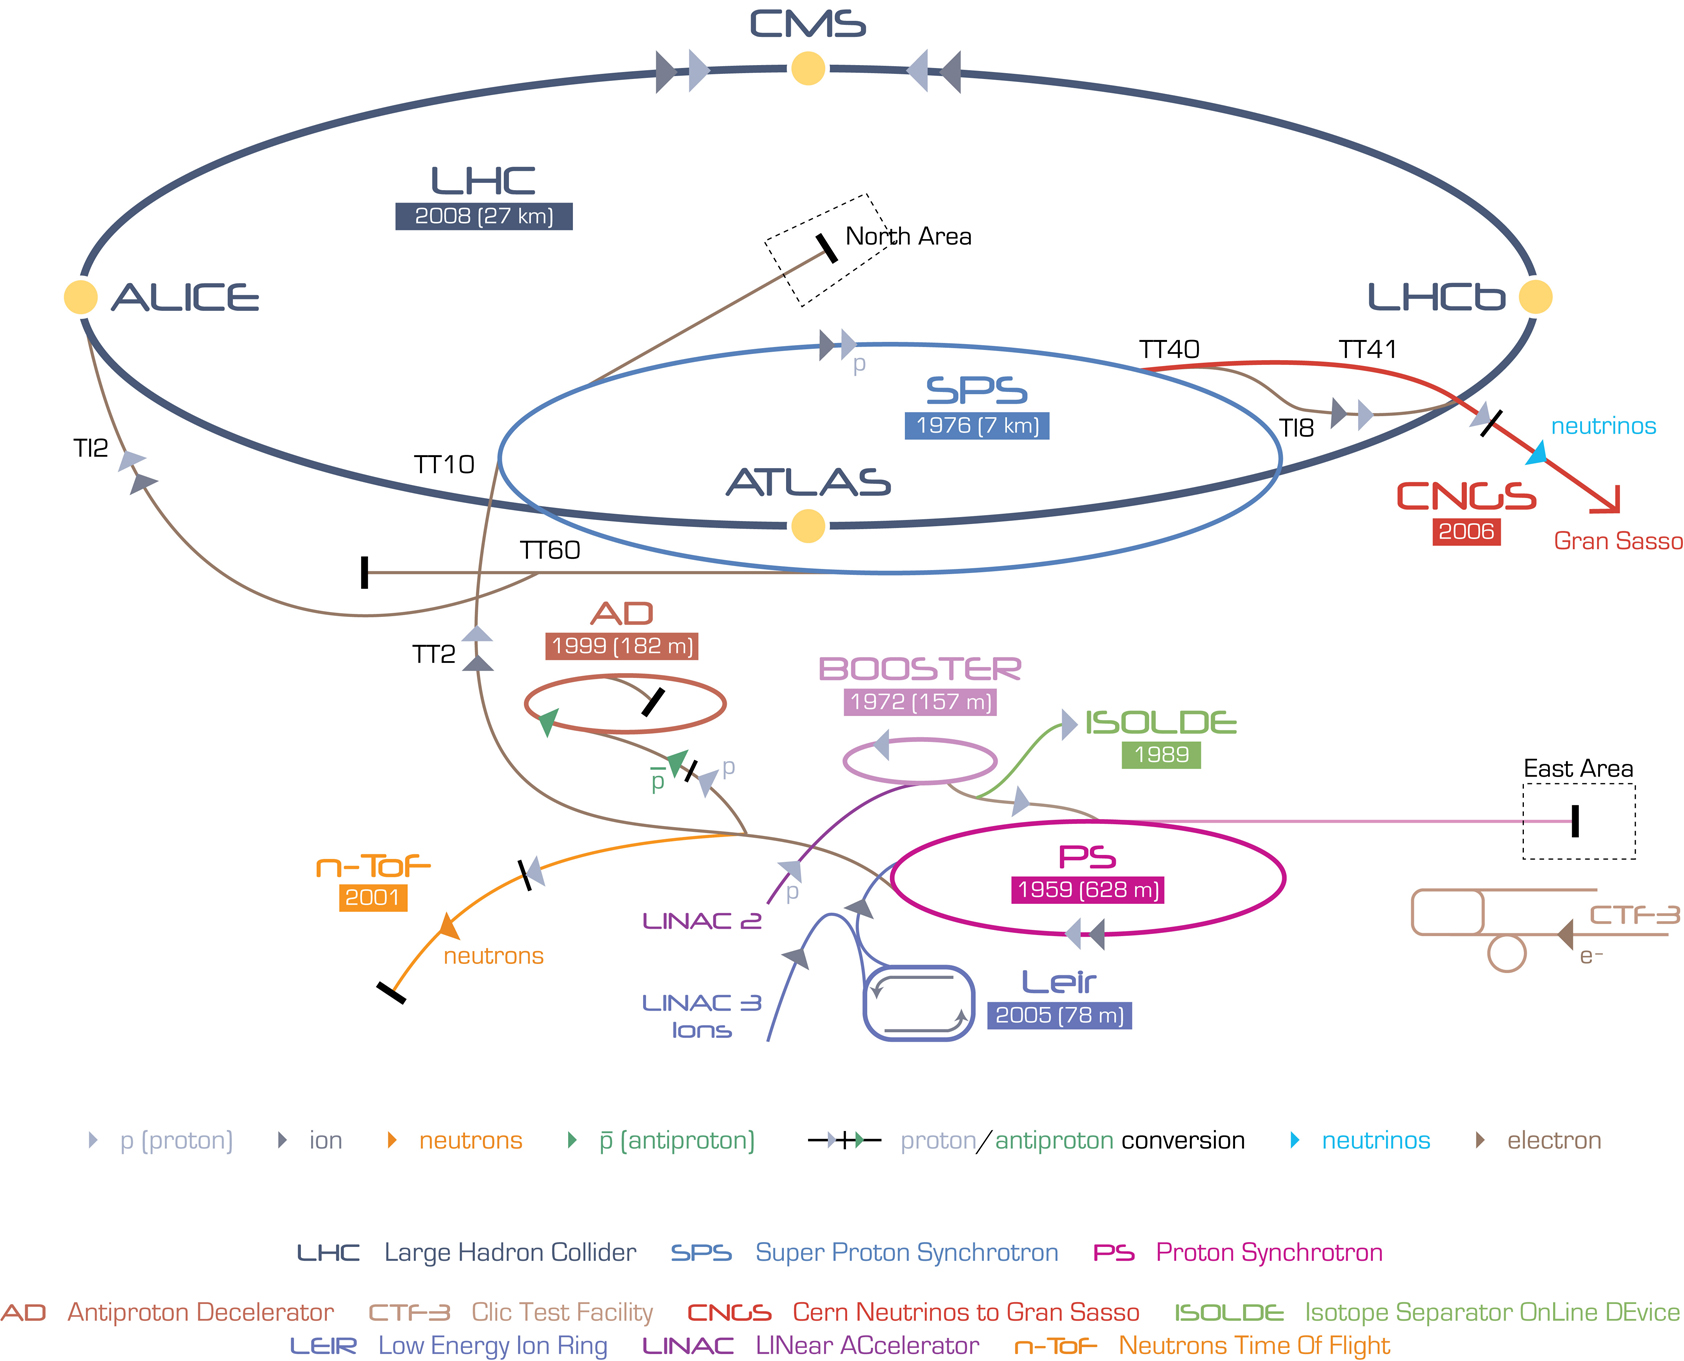
\includegraphics[width=0.6\textwidth]{figures/detector/Cern-Accelerator-Complex.jpg}
   \caption{A schematic view of the LHC ring~\cite{LHCReview}. LINAC2, Booster, PS, SPS, and LHC accelerate the protons in order. Four main experiments are located at interaction points along the ring. ATLAS and CMS are general purpose experiments, while ALICE focuses on heavy ion collisions and LHC$b$ is dedicated to $B$ physics.}
  \label{fig:LHC}
\end{figure}

\section{The Large Hadron Collider}
\label{sec:LHC}
\paragraph{}
Protons accelerated around the LHC originate in a red bottle of hydrogen gas. 
The $25$ minutes acceleration of the protons from rest to $6.5$ \TeV~ is accomplished in multiple steps:
\begin{itemize}
\item Electrons are stripped from the hydrogens to create protons;
\item A linear particle accelerator, Linac 2, accelerates the protons to $50$ \MeV; 
\item The Proton Synchrotron Booster (PSB) accelerates the protons to $1.4$ \GeV;
\item The Proton Synchrotron (PS) accelerates the protons to $25$ \GeV; 
\item The Super Proton Synchrotron (SPS) accelerates the protons to $450$ \GeV;
\item The $16.7$ kilometers LHC accelerates the protons to the final \TeV~ energies. 
%The LHC uses 1232 Niobium Titanium magnetic dipole for steering the protons. The magnets are cooled by superfluid helium to $1.9$ Kelvin, and can generate $8.33$ Tesla magnetic field.
\end{itemize}

\paragraph{}
The instantaneous luminosity, $L$ ($m^{-2}s^{-1}$), at the LHC is defined in Equation\ref{Ch2:eq-lumi} ~\cite{LHCReview}:
%
\begin{equation}
\label{Ch2:eq-lumi}
L = \frac{n_b N_b^2 f_{\rm rev} \gamma_r}{4\pi \epsilon_n \beta^*} F
\end{equation}
%
In the above Eq\ref{Ch2:eq-lumi}:
\begin{itemize}
	\item $n_b$ is the number of bunches per beam; %$n_b$ cannot be too large due to potential beam loss damages on the accelerator and detector; %Nominally, $2808$ proton bunches.
	\item $N_b$ is the number of protons per bunch;  
	\item $f_{\rm rev}$ is the proton revolution frequency;
	\item $\gamma_r$ is the relativistic Lorentz factor for the protons;
	\item $\epsilon_n$ is the normalized transverse beam emittance, or the average beam spread length;
	\item $\beta^*$ is the transverse beam size; $\sigma_{\rm beam} = \sqrt{\epsilon \cdot \beta}$; %affected by focusing magnets;
	\item $F$ is a reduction factor for the angle beams are colliding. %; smaller crossing angles could cause larger spread in the longitudinal direction.
\end{itemize}

\paragraph{} 
In $pp$ collisions, the rate of a certain physics process is $R_{\rm phy} = L\sigma$, where $\sigma$ ($m^2$) is the cross section.
The instantaneous luminosity can also be written as the ratio of the rate of inelastic collisions to the inelastic cross section $\sigma_{\rm inel}$ ~\cite{lumi-paper}:
\begin{equation}
\label{Ch2:eq-lumi2}
L = \frac{R_{\rm inel}}{\sigma_{\rm inel}} = \frac{\mu n_b f_{\rm rev}}{\sigma_{\rm inel}}
\end{equation}
where $\mu$ is the number of interactions per bunch crossing. 
For each bunch crossing, there is one main collision used for physics analysis with the highest center of mass energy, and many other lower energy collisions called ``pileup" interactions.
Larger ``pileup" requires higher detector resolution and faster reconstruction techniques.

\begin{table}[]
\centering
\caption[LHC nominal and operational parameters]{LHC nominal~\cite{LHCPaper} and operational parameters in 2015~\cite{LHC_2015} and 2016~\cite{LHC_2016}.}
\begin{tabular*}{\textwidth}{@{\extracolsep{\fill}}llll}
\hline
Parameter [unit]   & Nominal design value & 2015 Operating value  & 2016 Operating value\\
\hline\hline
Beam Energy [TeV]  & $7$  & $6.5$  & $6.5$  \\
Peak L [$10^{34} \text{cm}^{−2}~\text{s}^{-1}$]   & $1$ &   $0.5$  & $1.25$           \\
Bunch spacing [ns]             &      $25$  &  $25$ &      $25$ \\
$f_{\rm rev}$ [kHz]    &     $11245$  & $11245$  & $11245$ \\
$n_b$  [$10^{11}$ p/bunch]   & $1.15$ &  $1.15$ & $1.12$\\
$N_b$  [bunch]         & $2808$   &      $1825$ &      $2220$\\
$\epsilon_n$  [mm mrad]        & $3.5$ &  $3.5$  & $2$\\
$\beta^*$   [cm]         & $55$  &   $40$  & $40$\\
$F$        &      $0.84$  & $0.84$  &  $0.59$ \\
$\langle \mu \rangle$ & $19$ & $13$ & $41$ \\ \hline
\hline            
\end{tabular*}
\label{Ch2:tab-lhc}
\end{table}

\paragraph{}
The main parameters of the LHC beam and performance are shown in Table~\ref{Ch2:tab-lhc}. 
The target peak instantaneous luminosity for both the ATLAS and CMS experiments is $L=10^{34}~\text{cm}^{-2}\text{s}^{-1}$~\cite{LHCPaper}, which has already been exceeded in 2016. 
This is partly due to the improved $\beta^*$ and $F$.
The number of ``pileup" interactions also increases, shown in Figure~\ref{fig:Mu_2015_2016}. 

\begin{figure}[htbp!]
  \centering
  \captionsetup{justification=centering}
  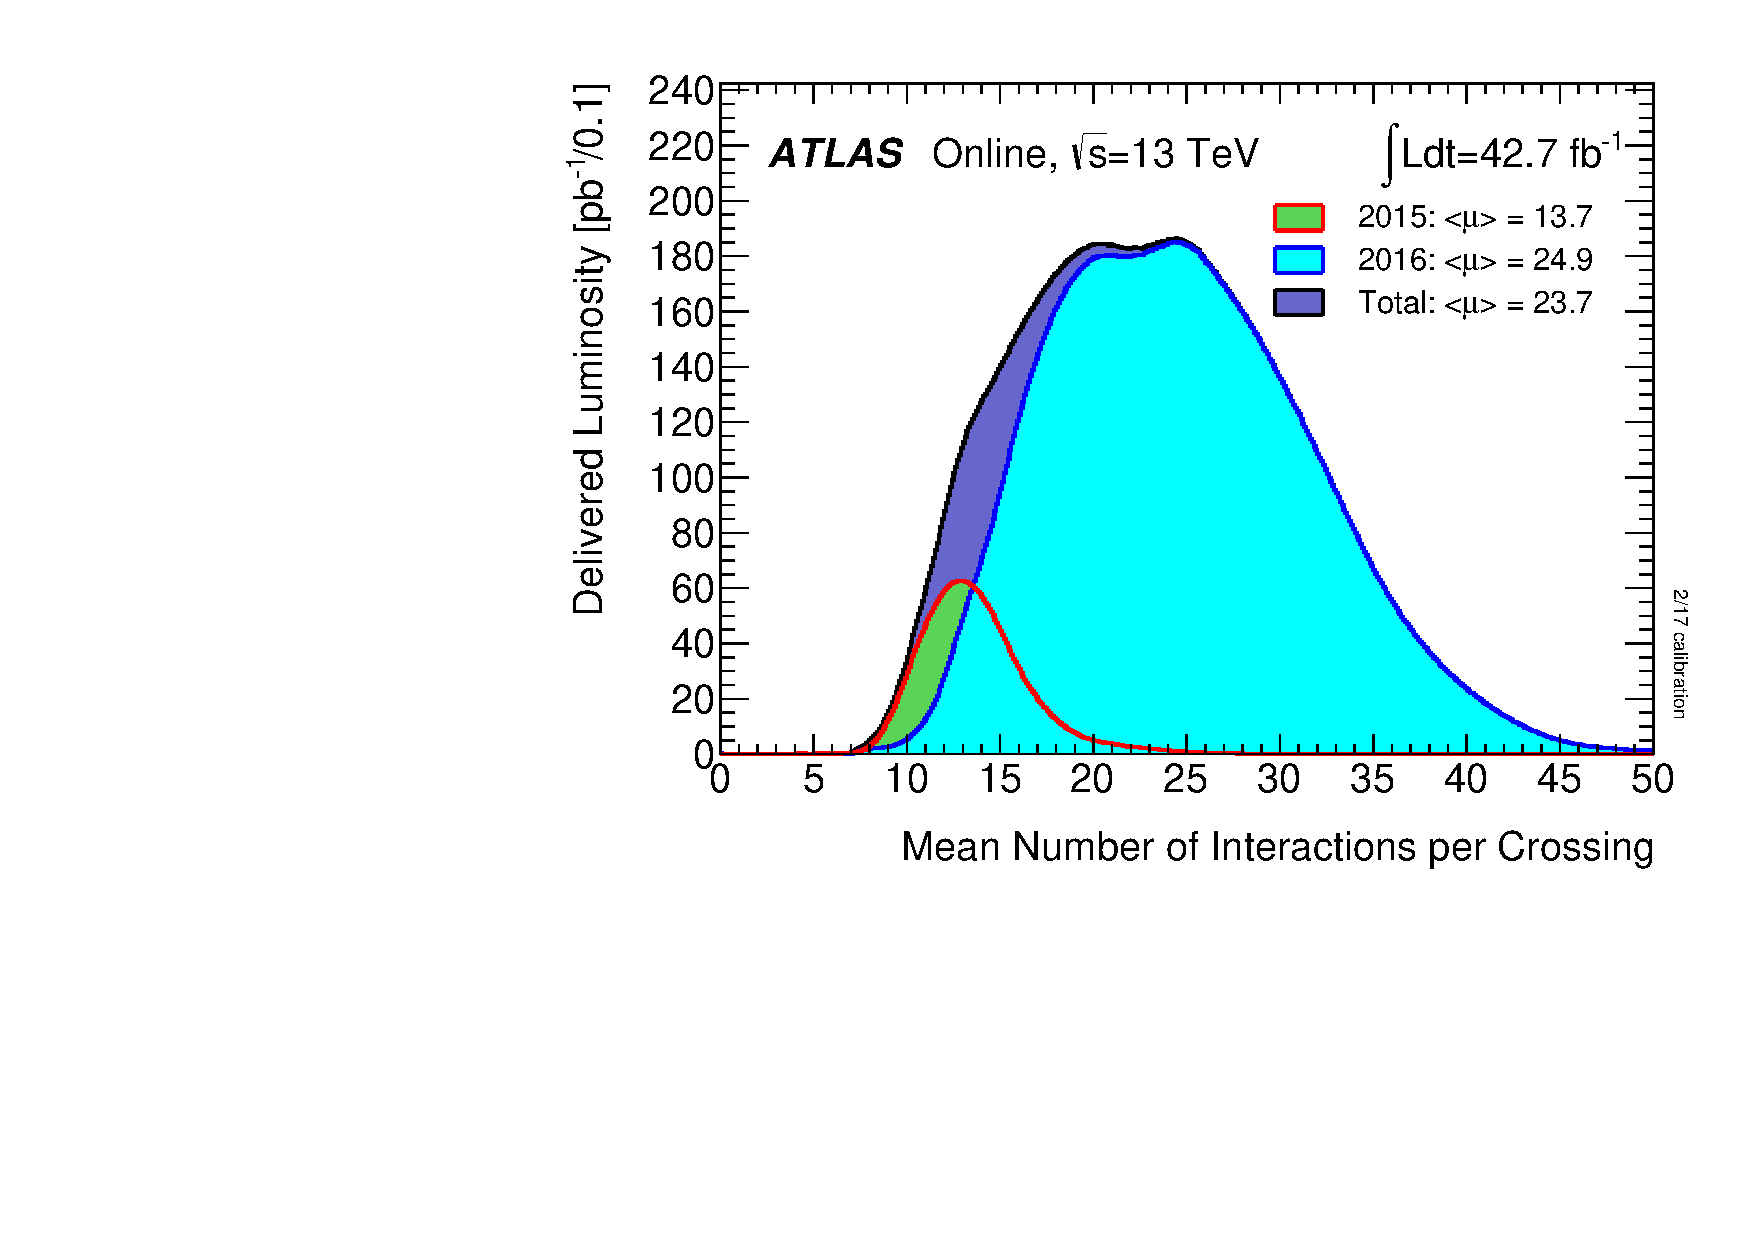
\includegraphics[width=0.5\textwidth,angle=-90]{figures/detector/Mu_2015_2016}
   \caption{The luminosity-weighted distribution of the mean number of interactions per crossing for the 2015 and 2016 $pp$ collision data at $13$ \TeV center-of-mass energy.~\cite{Lumi_Run2}}
  \label{fig:Mu_2015_2016}
\end{figure}
%At the nominal LHC conditions, the beam energy is about 360 MegaJoules, and the LHC in total consumes 115 MegaWatt of power.


\section{A Toroidal LHC ApparatuS}
\label{sec:ATLAS}

\paragraph{}
The ATLAS experiment~\cite{PERF-2007-01} at the LHC is a general-purpose particle detector with a near $4\pi$ coverage in solid angle and a forward-backward symmetric cylindrical geometry. 
The ATLAS detector (Figure~\ref{fig:ATLAS}) consists of an inner tracking detector (ID) surrounded by a $2.3$ m diameter thin superconducting solenoid providing a $2$T axial magnetic field, electromagnetic (EM) and hadronic calorimeters, and a muon spectrometer (MS). Three extra air-core toroid magnets generate the magnetic field in the MS. 
%with $1.5$ to $5.5 ~\textrm{T} \cdot\textrm{m}$ of bending power at $0<|\eta|<1.4$ and approximately $1$ to $7.5 ~\textrm{T} \cdot\textrm{m}$ in the endcap region of $1.6 < |\eta| < 2.7$.

\begin{figure}[htbp!]
  \centering
  \captionsetup{justification=centering}
  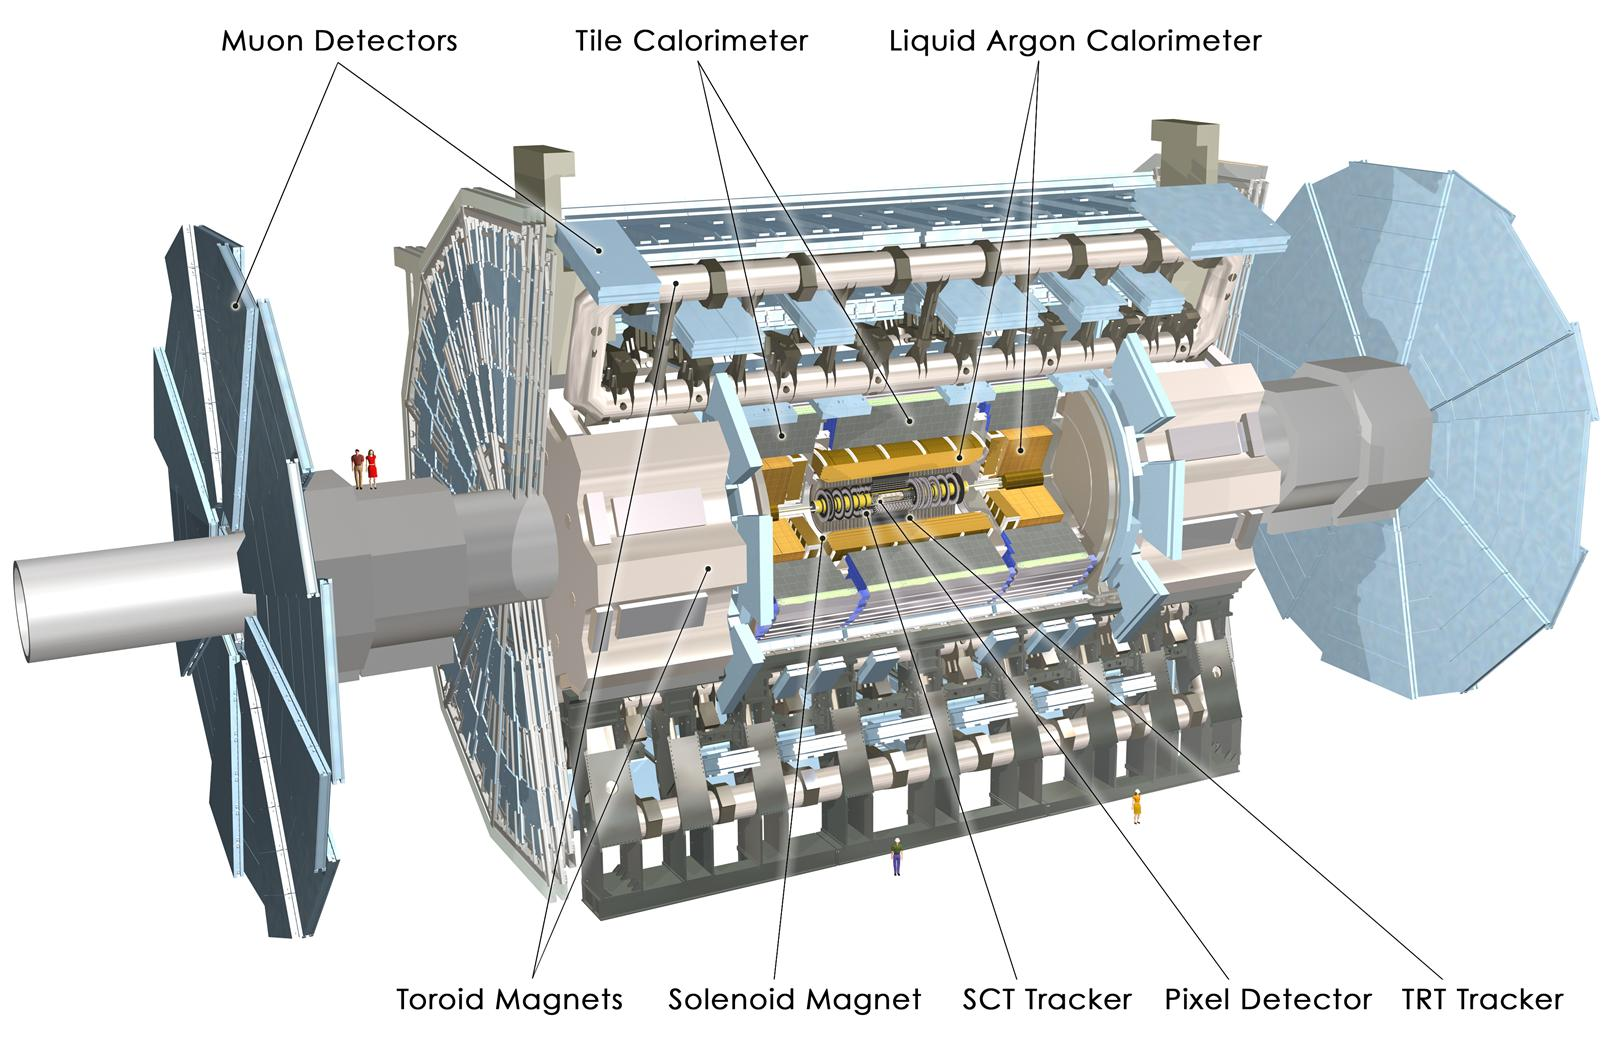
\includegraphics[width=0.7\textwidth]{figures/detector/ATLAS.jpg}
   \caption{A detailed computer-generated image of the ATLAS detector and it's systems.}
  \label{fig:ATLAS}
\end{figure}

%%%%%%%%%%%%%%
\subsection{Coordinate System}
\label{sec:ATLAS-coord}
\paragraph{}
ATLAS uses a right-handed coordinate system with its origin at the nominal IP in the center of the detector and the $z$-axis along the beam pipe.
The positive $x$-axis points from the IP to the center of the LHC ring, the positive $y$-axis points towards the sky, and the $z$-axis points straight (like bridges) towards the Geneva airport (A side), back from the Charlie's pub in France (C side).
Cylindrical coordinates $(r,\phi)$ are used in the transverse plane, $\phi$ being the azimuthal angle around the $z$-axis.
The pseudorapidity is defined in terms of the polar angle $\theta$ as $\eta = -\ln \tan(\theta/2)$. $\eta$ the massless approximation of rapidity $y = \frac{1}{2} \ln \frac{E + p_{z}}{E - p_{z}}$.
$\theta$ is the angle parameterizing special relativity's boosts along the $z$-axis. 
%Most hadron productions are roughly constant in $\eta$, and for two massless particles traveling in different directions, their difference in $\Delta \eta$ is invariant. 
The angular distance is measured in units of $\Delta R = \sqrt{(\Delta\eta)^{2} + (\Delta\phi)^{2}}$.

\paragraph{}
The region with $|\eta| < 1.5$ is called the ``central" region. 
It consists of the ``barrel" elements, which are arranged in a cylindrical fashion around the beam line.
In the ``endcap" region, with $|\eta| > 1.5$, the detector elements are arranged as disks perpendicular to the beam line.
The ``forward" region of the detector has $|\eta| > 2.5$.

%%%%%%%%%%%%%%
\subsection{Inner Detector}
\paragraph{}\
The ID is important for track reconstruction and heavy flavor $b$-tagging. 
The ID covers the pseudorapidity range $|\eta| < 2.5$.
It consists of three sub-detectors: the silicon pixel detector (PIXEL), the silicon microstrip detector (SCT), and the straw-tube transition-radiation tracking detector (TRT) . 
An additional pixel detector layer (IBL) ~\cite{Capeans:1291633}, positioned at a mean radius of $3.3$ cm, is inserted before the Run-2 data-taking and improves the identification of $b$-jets~\cite{ATL-PHYS-PUB-2015-022}. 
A $10$\GeV~ charged particle in the barrel region will produce $1$ IBL hits, $3$ PIXEL hits, $8$ SCT hits and $36$ TRT hits.
Figure~\ref{fig:Det_ID_rz} ~\cite{Aaboud:2017pjd} shows the $R$-$z$ distribution of the material for a quadrant of the barrel region PIXEL and SCT. 
Figure~\ref{fig:Det_ID_xy} shows the distribution of hadronic-interaction vertex candidates in $|\eta|<2.4$ and $|z|<400$ mm for $13$\TeV~ data.

%\paragraph{}
%The ID is designed to provide charged particle momentum measurement with $\sigma_{p_{T}}/p_{T} \sim 0.05\% p_{T} \oplus 1\%$ and vertex reconstruction.
%Because of this, each detector proves measurement accuracies of the order $10 \mu\rm m$ in $R$-$\phi$ and $100 \mu\rm m$ in $z$.
%The intensity of a particle beam decreases exponentially in radiation length. $I(x) = I_0 e^{-x/X_0}$, where $I$ is the intensity, $x$ is the distance traveled, and $X_0$ is the radiation length.

\begin{figure}[htbp!]
\centering
\captionsetup{justification=centering}
    \begin{subfigure}[b]{0.6\textwidth}
        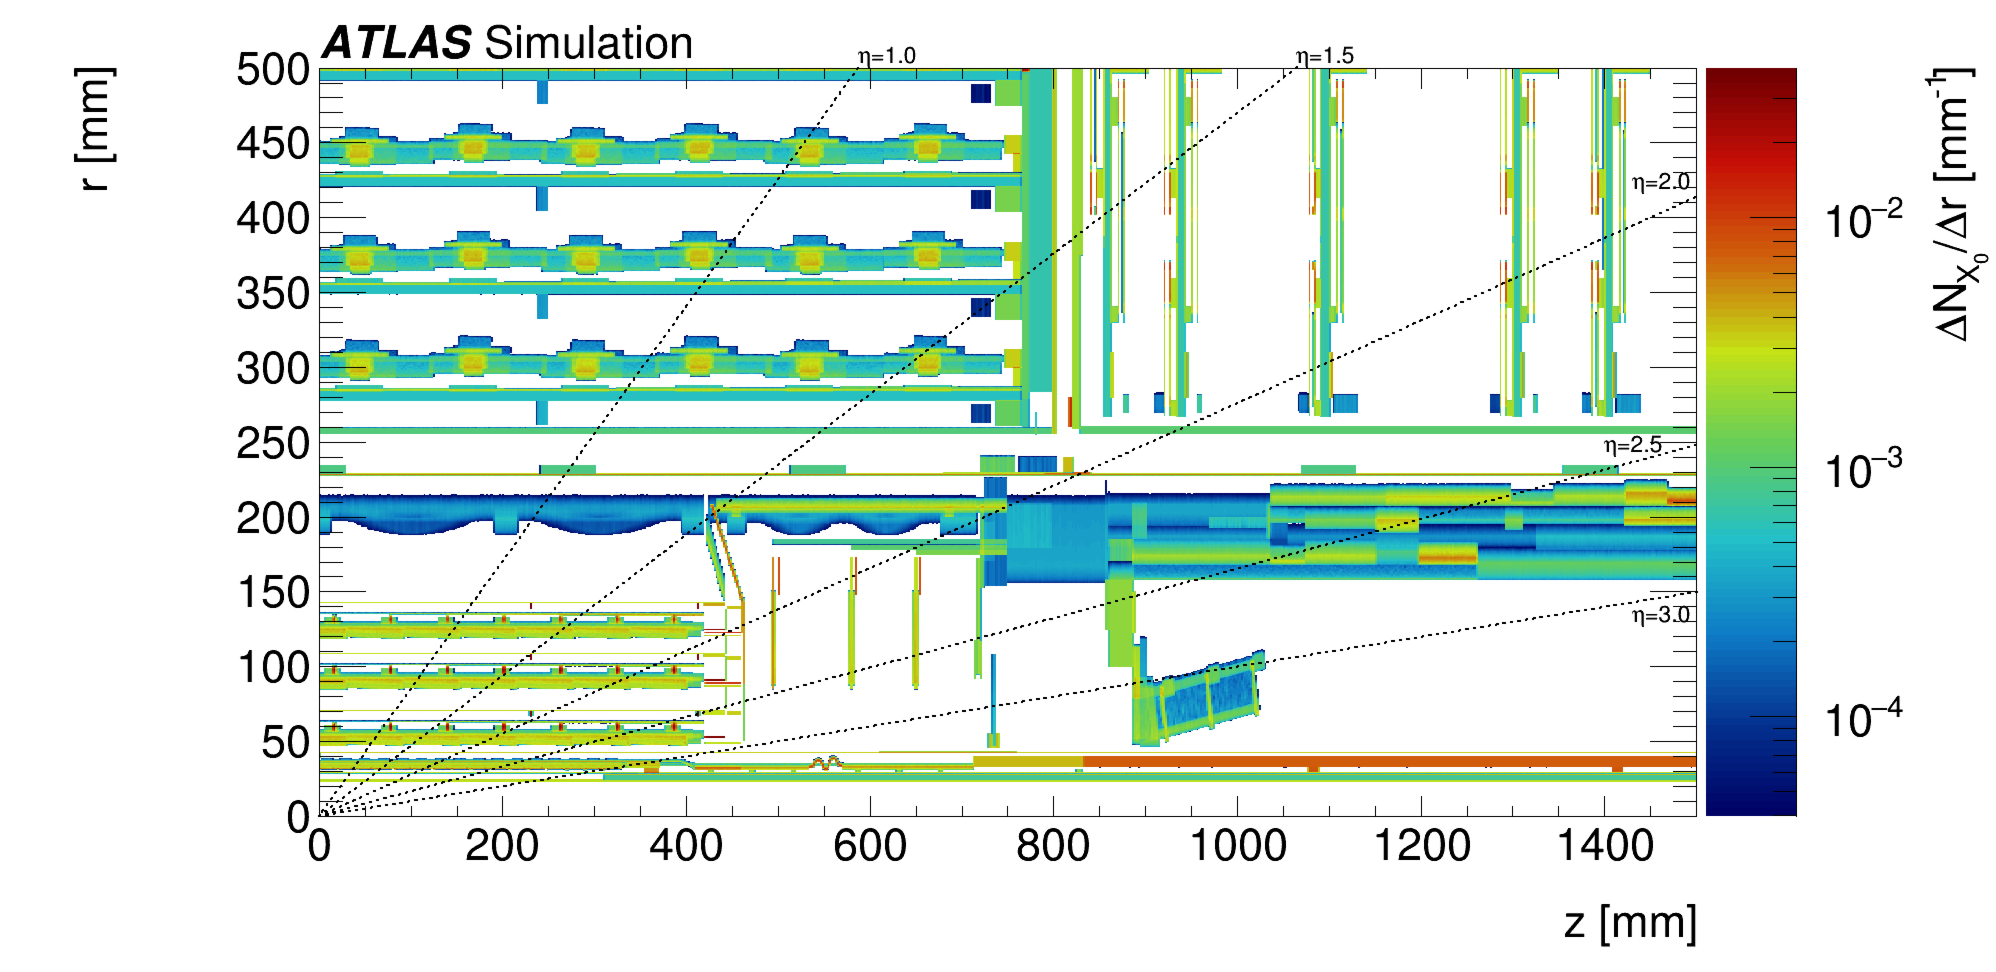
\includegraphics[width=\textwidth]{figures/detector/ID_rzmap}
        \caption{The $R$-$z$ distribution of material's differential number of radiation lengths, $\frac{\Delta N_{X_0}}{\Delta r}$}
        \label{fig:Det_ID_rz}
    \end{subfigure}
    \quad
    \begin{subfigure}[b]{0.3\textwidth}
        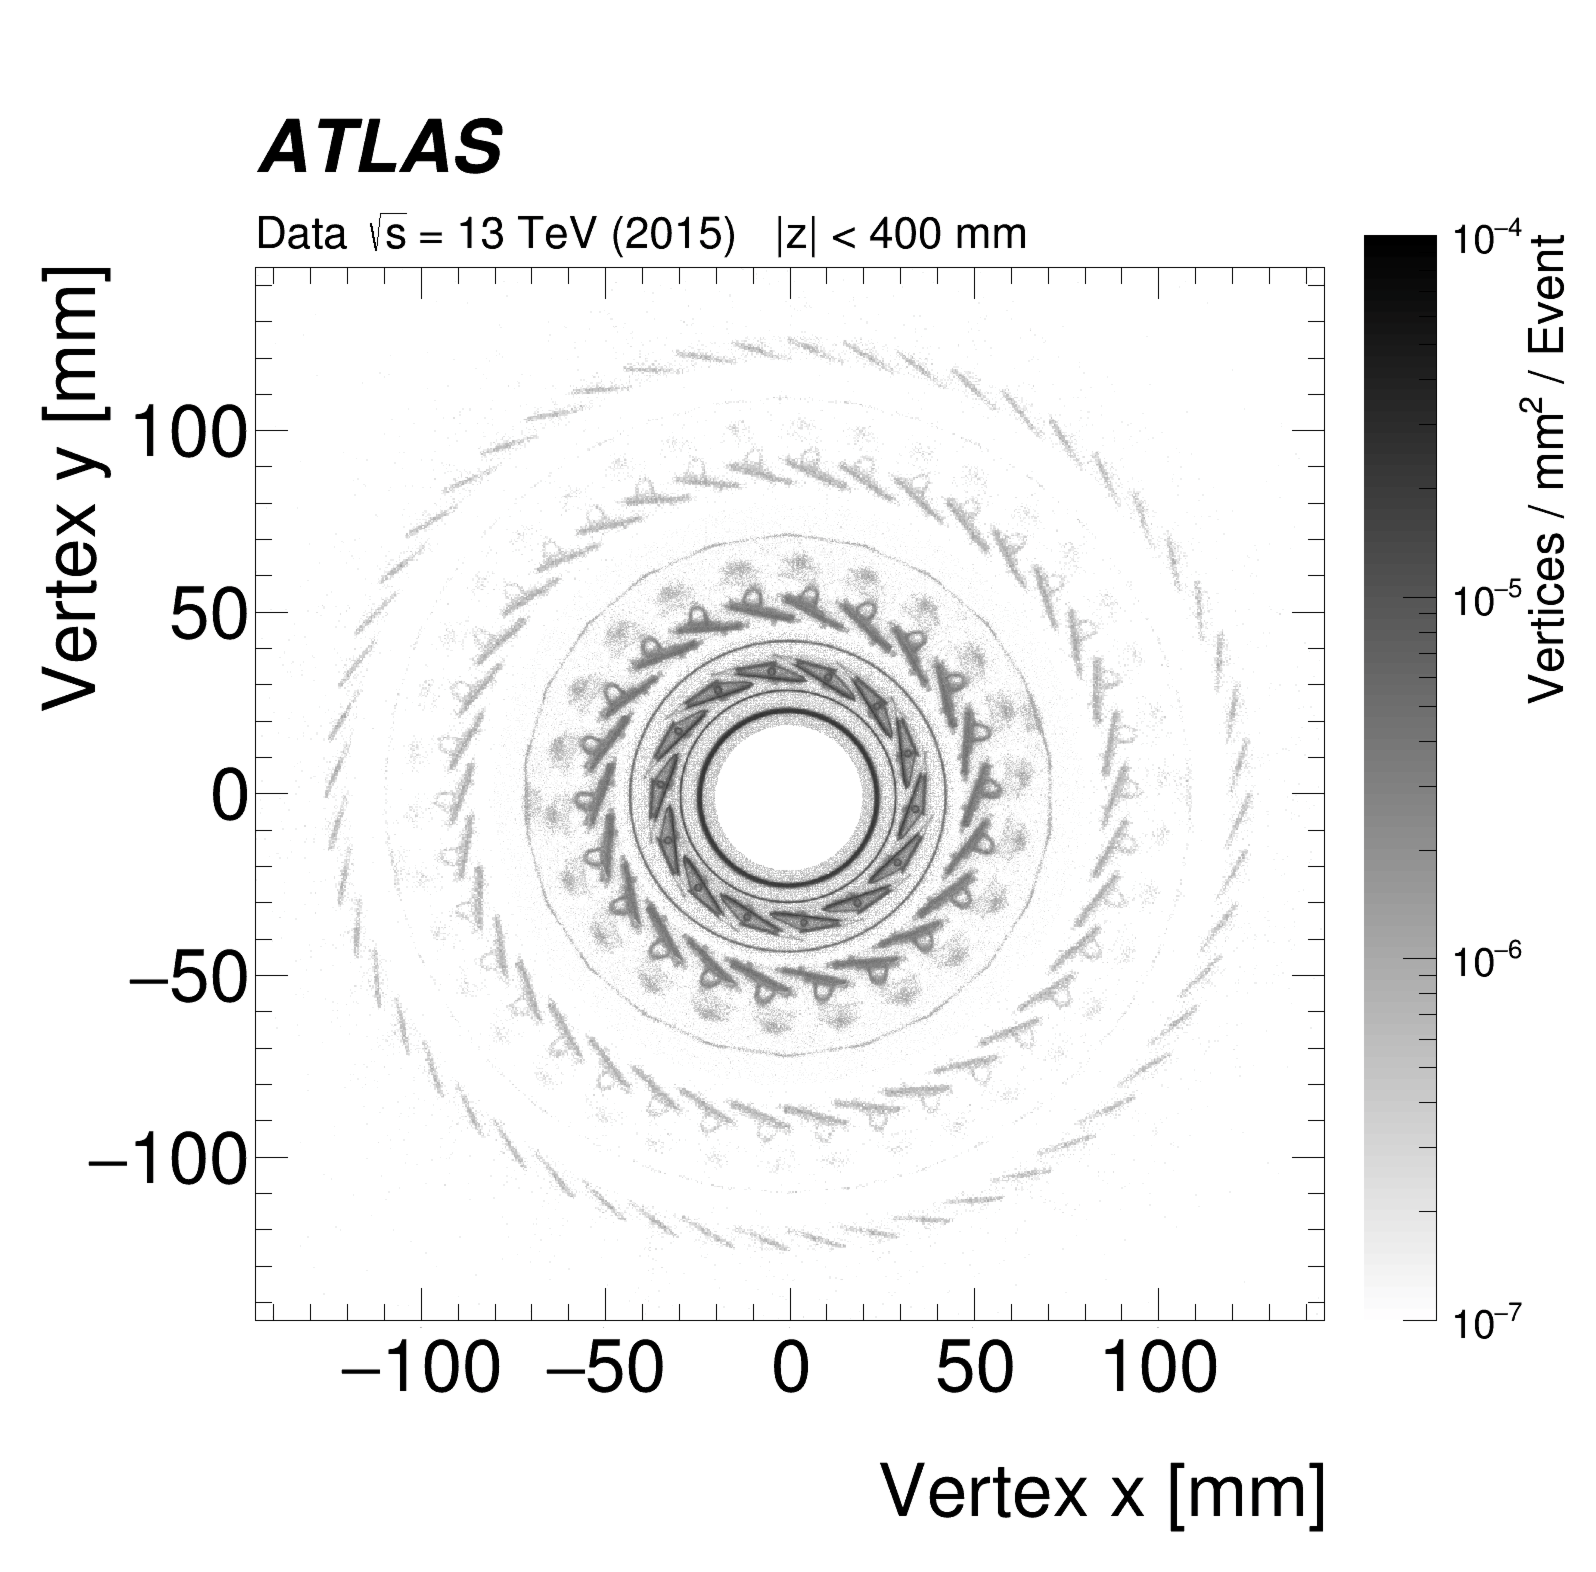
\includegraphics[width=\textwidth]{figures/detector/ID_data_map_XY}
        \caption{Distribution of hadronic-interaction vertex candidates}
        \label{fig:Det_ID_xy}
    \end{subfigure}
\caption{Geometry of IBL, PIXEL and SCT detectors in Run2.}
\label{fig:Det_ID}
\end{figure}

%Material of ATLAS Inner Detector for Run 2 of the LHC. \href{https://cds.cern.ch/record/2260595/files/PERF-2015-07-002.pdf}{note}.
%%%%%%%%%%%%%%
\subsection{Calorimeter}
\paragraph{}
The calorimeters are important for measuring the energy of the Higgs boson decay productions.
A lead and liquid argon (LAr) sampling calorimeter with finely segmented layers provides EM energy measurements.
A steel/scintillator-tile hadronic calorimeter covers the central pseudorapidity range ($|\eta| < 1.7$) and provides hadronic energy measurements.
The endcap and forward regions are instrumented with copper/tungsten and LAr calorimeters for both the EM and hadronic energy measurements up to $|\eta| = 4.9$. 
The calorimeters also provide basic EM/hadronic trigger information, with fast analog summing in coarse granularity.

%\paragraph{}
%EM calorimeter (ECal) is designed to have $>22$ radiation lengths in the barrel and $> 24$ in the endcap. 
%It provides EM measurement with $\sigma_E/E = 10\%/\sqrt{E} \oplus 0.7\%$. The hadronic calorimeter (HCal) has approximately $9.7$ interaction length in the barrel and $10$ in the endcap. 
%HCal provides hadronic measurement with $\sigma_E/E = 50\%/\sqrt{E} \oplus 3\%$ in the Barrel and Endcap regions, and $\sigma_E/E = 100\%/\sqrt{E} \oplus 10\%$  in the forward region.

%%more plots: https://twiki.cern.ch/twiki/bin/view/AtlasPublic/LArCaloPublicResults2015

%%%%%%%%%%%%%%
\subsection{Muon Spectrometer}

\begin{figure}[htbp!]
\centering
\captionsetup{justification=centering}
    \begin{subfigure}[b]{0.5\textwidth}
        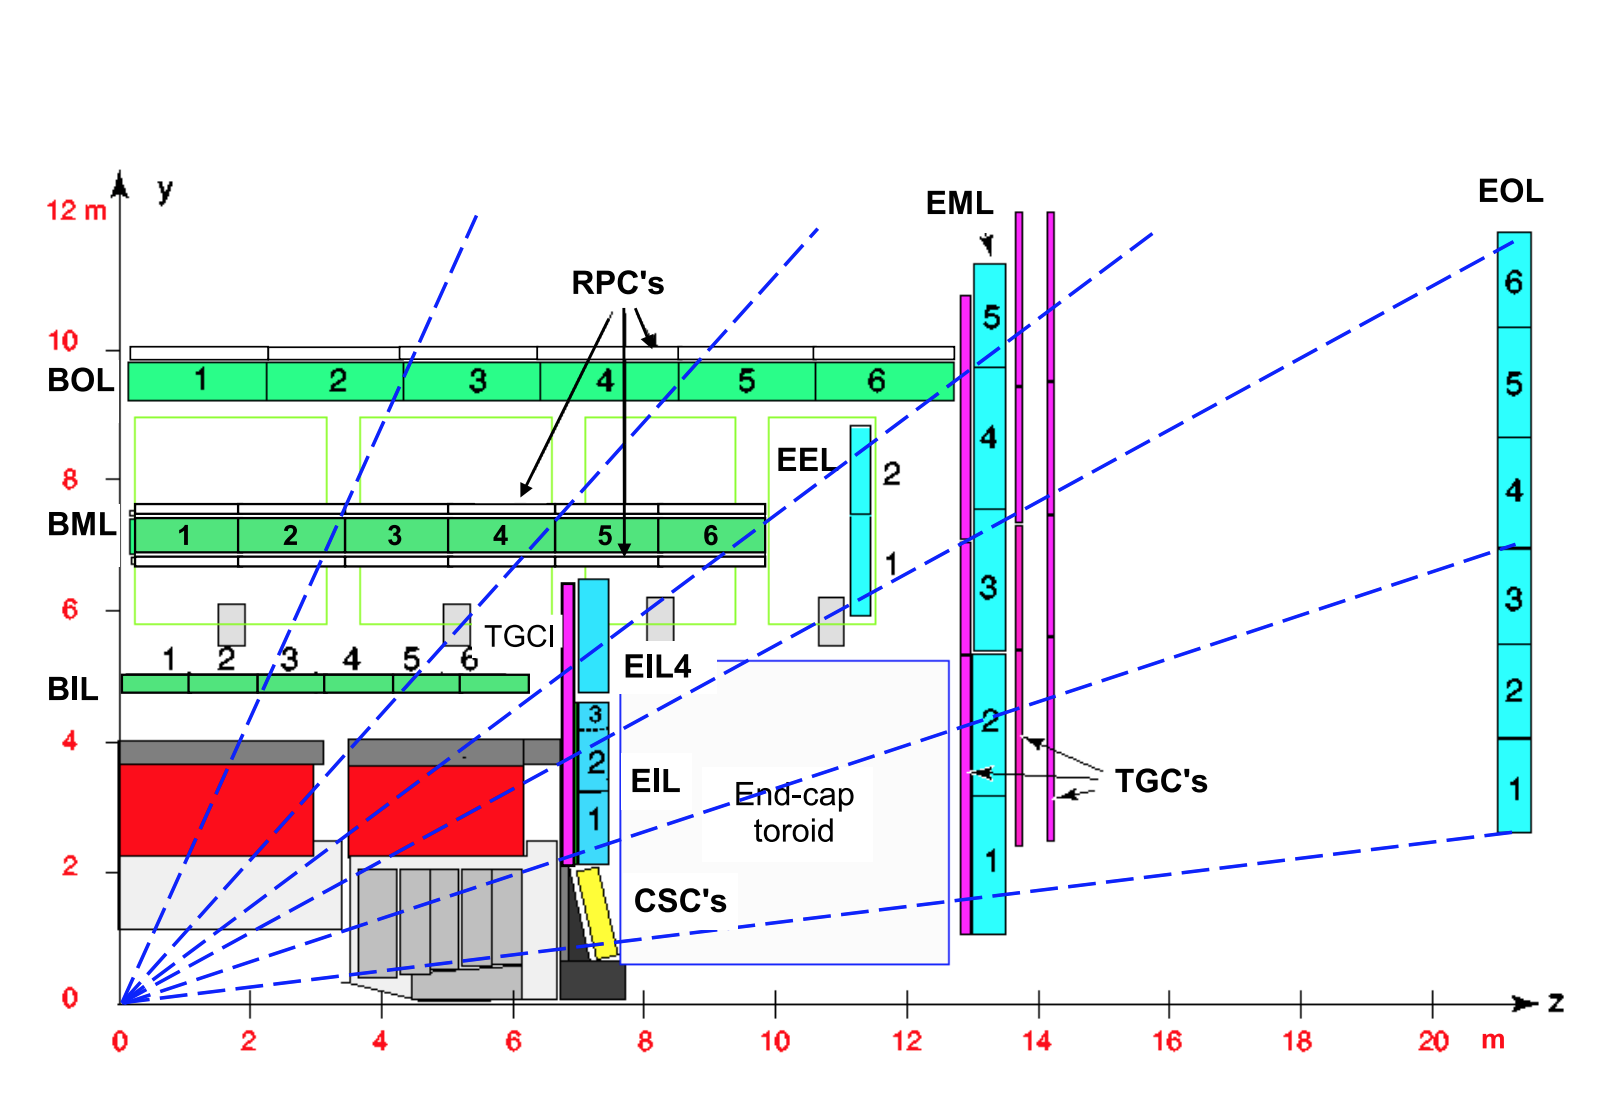
\includegraphics[width=\textwidth]{figures/detector/MS_rz}
        \caption{Cross-section of the muon system in $R$-$z$ plane. Numbers indicate different $\eta$ stations. For MDT letters, B means barrel, and E means endcap. I stands for inner, M for middle, O for outer, and E for extra.}
        \label{fig:MS_rz}
    \end{subfigure}
    \quad
    \begin{subfigure}[b]{0.3\textwidth}
        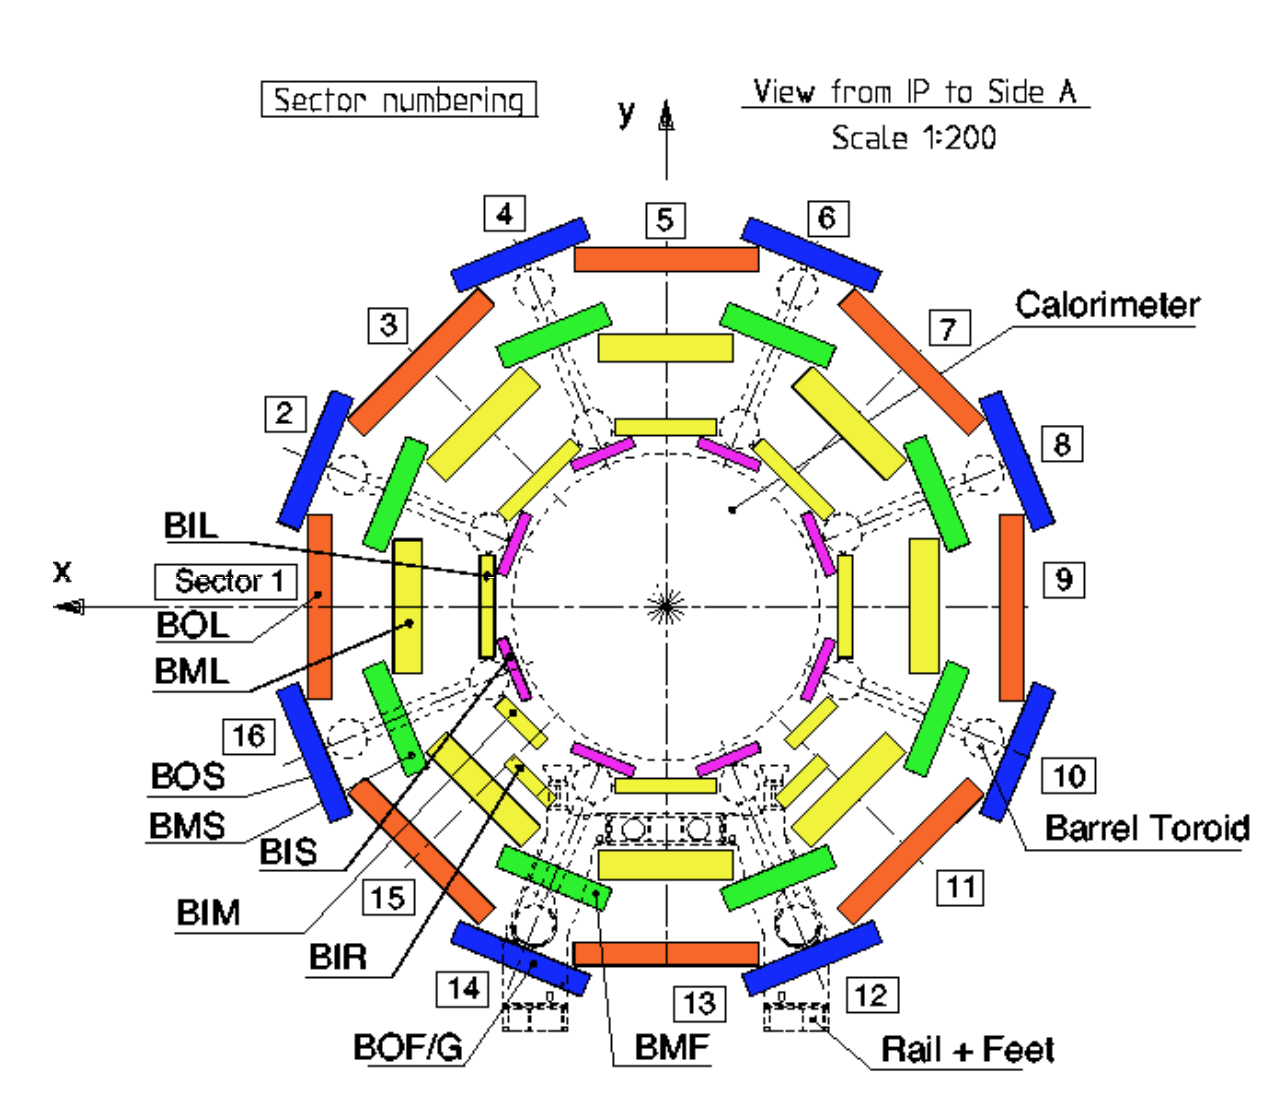
\includegraphics[width=\textwidth]{figures/detector/MS_phi}
        \caption{Cross-section of the barrel muon system in $x$-$y$ plane. Numbers indicate different $\phi$ stations. Last L means large sectors and last S means small sectors.}
        \label{fig:MS_phi}
    \end{subfigure}
\caption{The overall layout of the ATLAS MuonSpectrometer.}
\label{fig:Det_MS}
\end{figure}

\paragraph{}
The muon spectrometer (Figure~\ref{fig:Det_MS}) is the largest component of the ATLAS detector.
It surrounds the calorimeters and includes three large superconducting air-core toroids. 
The field integral of the toroids ranges between 2 and 6 T/m for most of the detector. Because of this bending power, the MS measures muon momentum stand-alone, with $\sigma_{p_{T}}/p_{T} \sim 10\%$ at $p_{T} = 1$\TeV. 
Muon Drift Tubes (MDT) and Cathode Strip Chambers (CSC) are the precision tracking detectors. 
%Each MDT has $80\,\mu\textrm{m}$ single hit spacial resolution, with an alignment precision of $30\,\mu\textrm{m}$.
Resistive Plate Chambers (RPC) in the barrel and Thin Gap Chambers (TGC) are the triggering detectors, with $1.5$-$5$ ns timing resolution. 

%%%%%%%%%%%%%%
\subsection{Trigger and Data Acquisition}
\paragraph{}
A dedicated trigger system is used to select interesting physics collision events~\cite{ATLAS-TRIGGER}.
The first-level trigger (L$1$) is implemented in hardware and uses the calorimeter and muon detectors to seed regions of interest (RoI) and reduce the accepted event rate to $100$ kHZ.
This is followed by a software-based high-level trigger (HLT) that reduces the accepted event rate to $1$ kHZ on average. 
To avoid high rates for certain triggers, the triggers are often prescaled, which means some accepted events get rejected. 
For example, a prescale of two means only every second event passing all trigger conditions gets accepted. 

\paragraph{}
Over 2015 and 2016, both the LHC and the ATLAS performed outstandingly ~\cite{Lumi_Run2}. The total data recording efficiency for ATLAS is around $92\%$, shown in Figure~\ref{fig:Lumi}.

\begin{figure}[htbp!]
\centering
\captionsetup{justification=centering}
	\hspace{-2cm}
    \begin{subfigure}[b]{0.35\textwidth}
        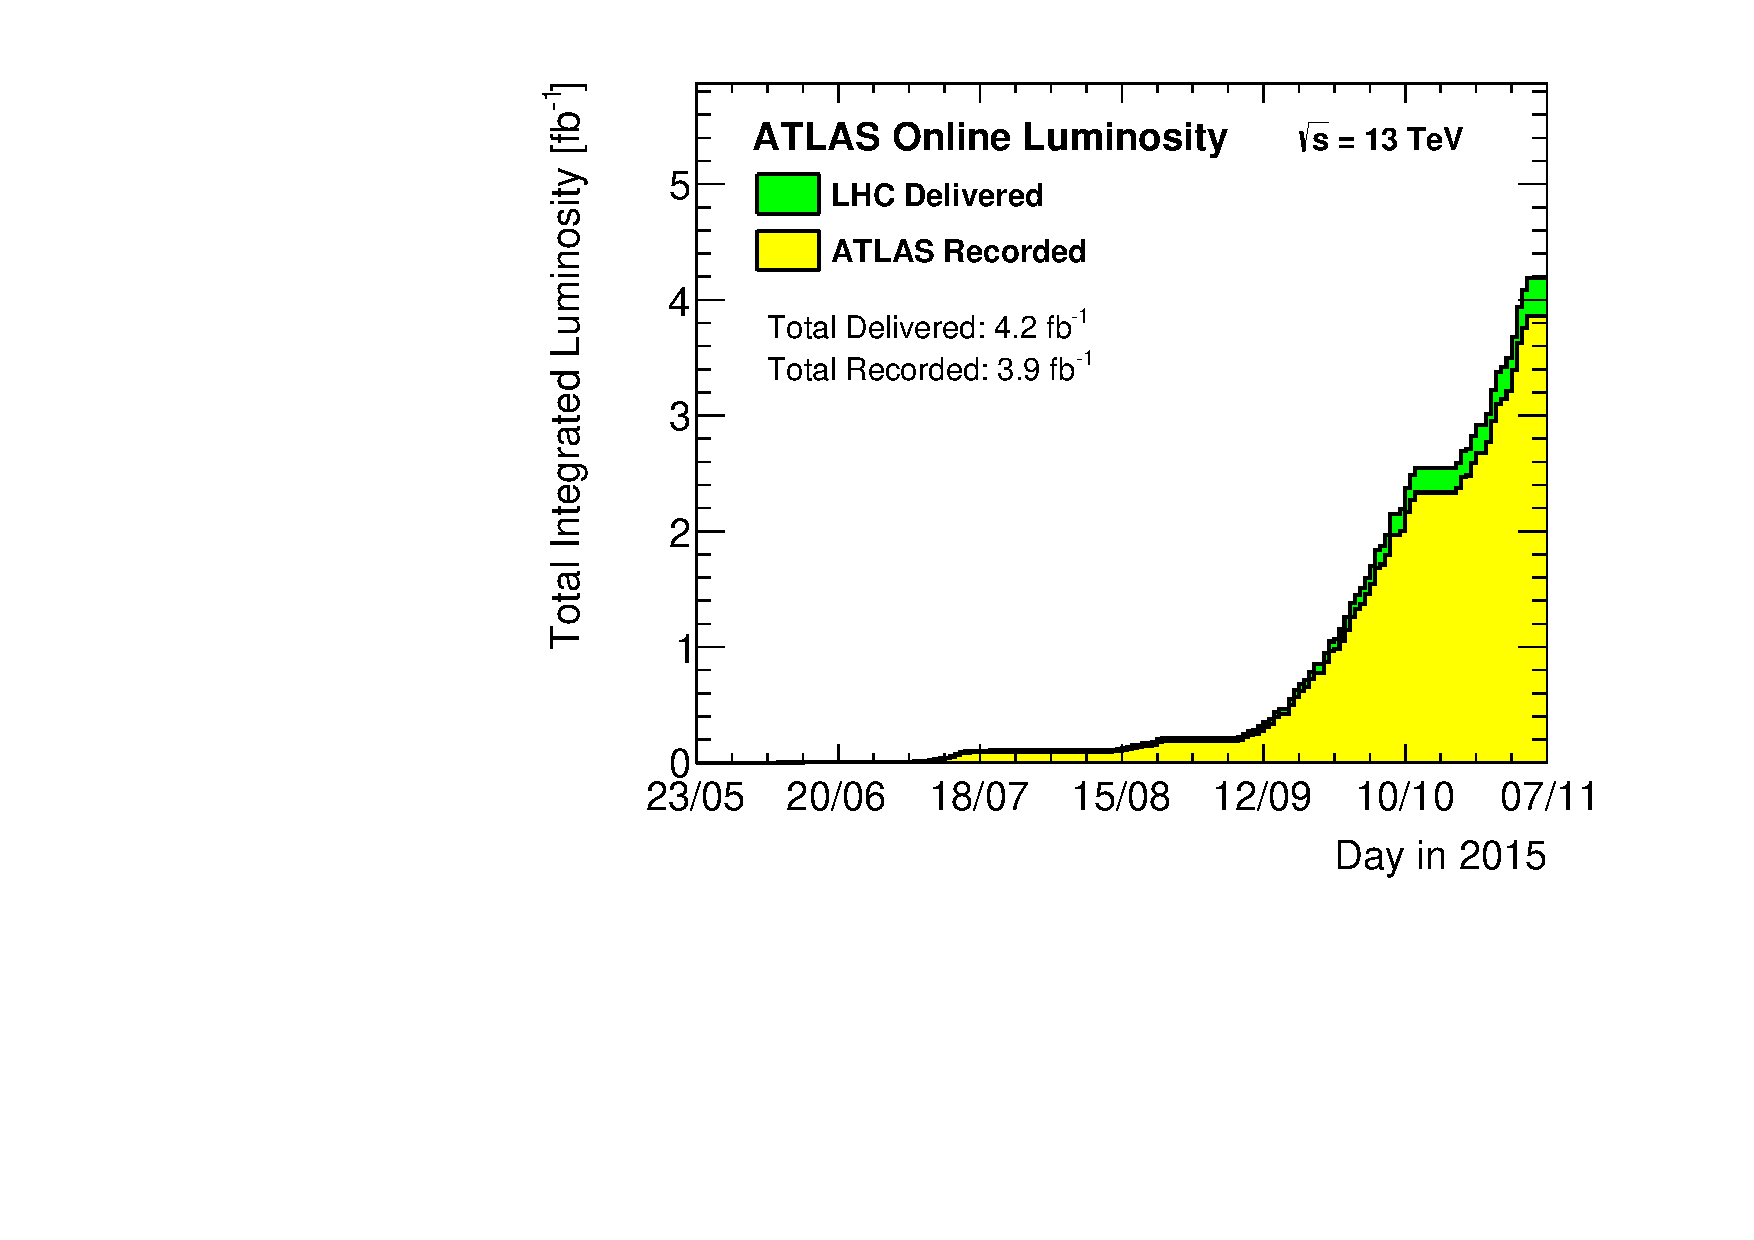
\includegraphics[width=\textwidth,angle=-90]{figures/detector/Lumi_2015}
        \caption{2015}
        \label{fig:Lumi_2015}
    \end{subfigure}
    \quad
    \quad
    \quad
    \quad
    \begin{subfigure}[b]{0.35\textwidth}
        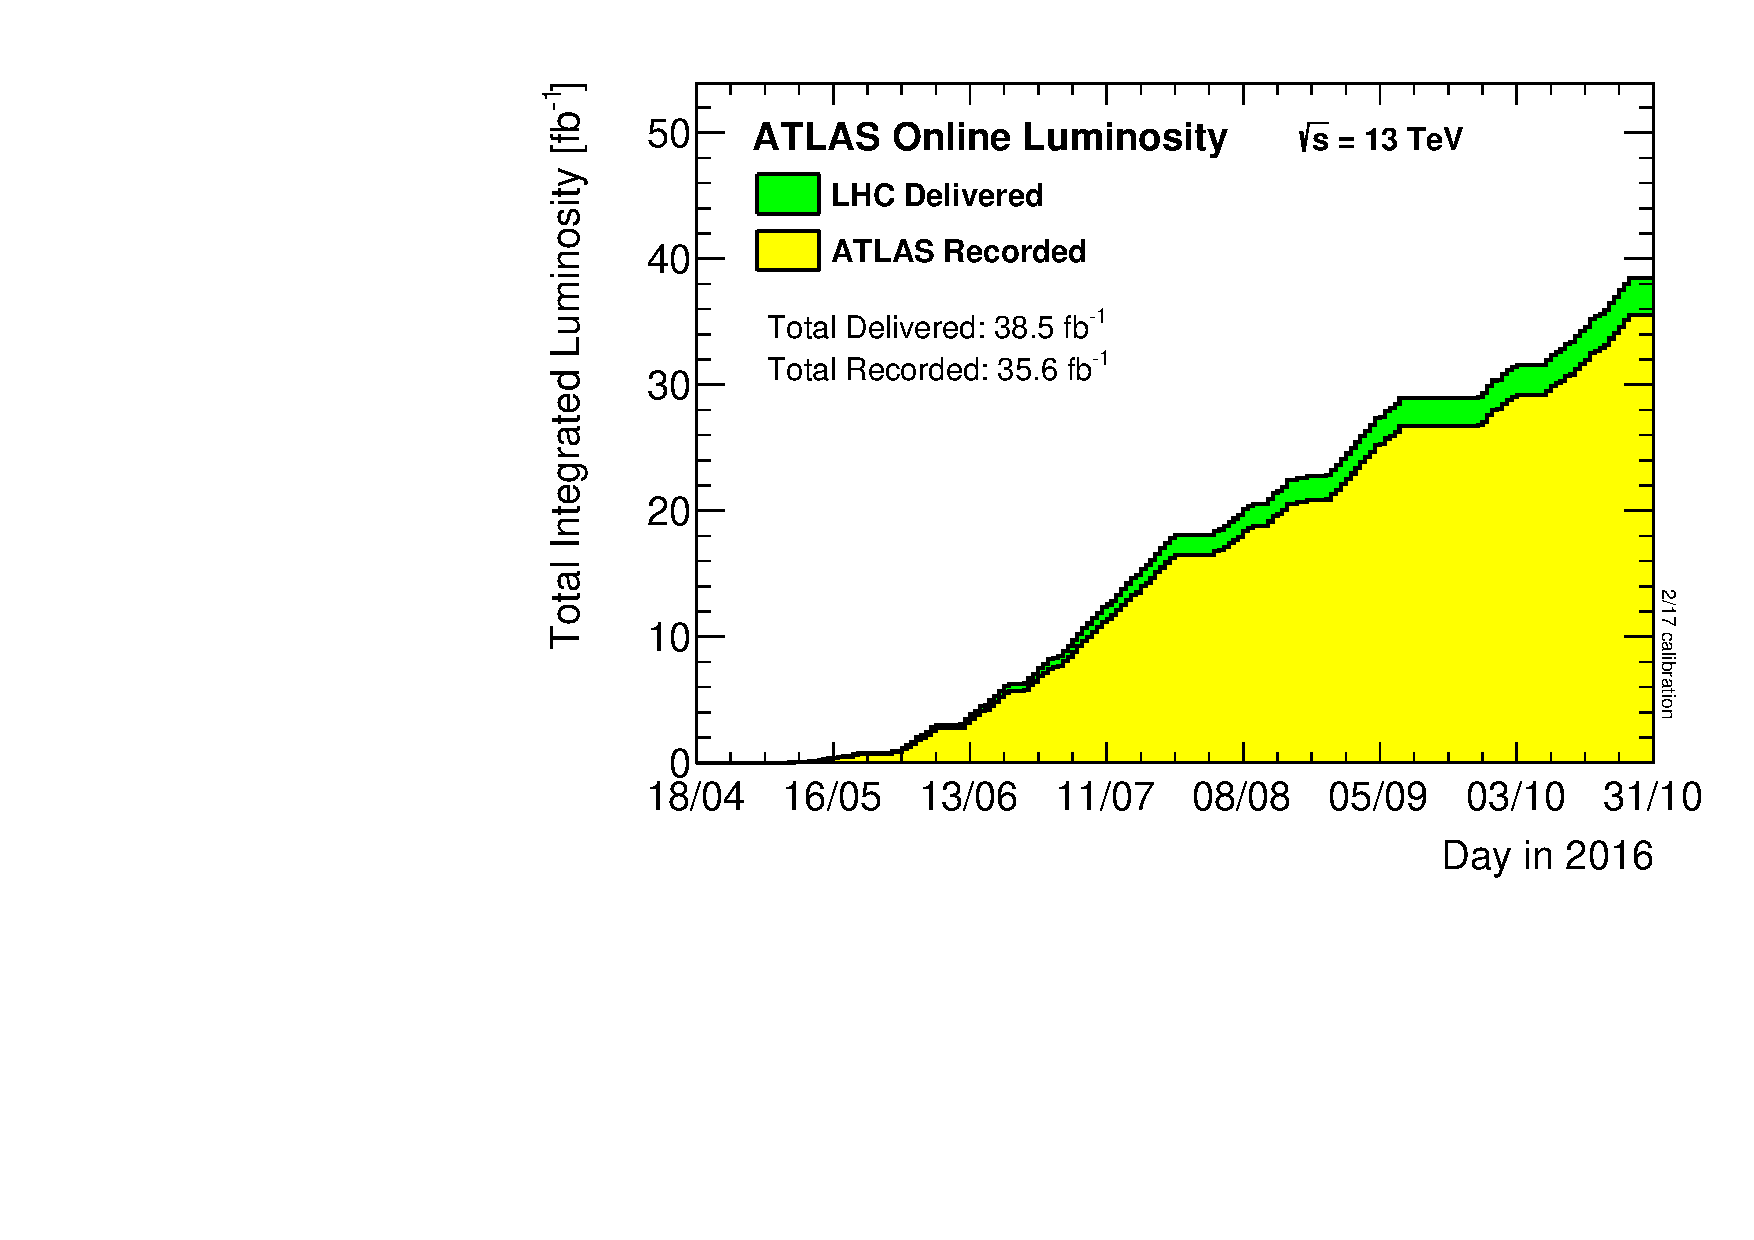
\includegraphics[width=\textwidth,angle=-90]{figures/detector/Lumi_2016}
        \caption{2016}
        \label{fig:Lumi_2016}
    \end{subfigure}
\caption{Cumulative luminosity vs. time delivered to (green) and recorded by ATLAS (yellow) during stable beams for $pp$ collisions at $13$ \TeV center-of-mass energy.}
\label{fig:Lumi}
\end{figure}

% \paragraph{}
% For further trigger information, see \href{http://atlas.web.cern.ch/Atlas/GROUPS/PHYSICS/PAPERS/TRIG-2016-01/}{2015 note} and \href{https://cds.cern.ch/record/2242069/files/ATL-DAQ-PUB-2017-001.pdf}{2016 updates}.





